\documentclass[sigconf,review,anonymous]{acmart}


%% ── Packages ──────────────────────────────────────────────────────────────────
\usepackage{booktabs}
\usepackage{multirow}
\usepackage{makecell}
\usepackage{amsmath}
\let\Bbbk\relax
\usepackage{amssymb}
\usepackage{graphicx}
\usepackage{microtype}
\usepackage{xcolor}
\usepackage{listings}
\usepackage{tikz}
\usetikzlibrary{positioning,calc,arrows.meta}
\usepackage{pgfplots}
\pgfplotsset{compat=1.18}


%% ── Convenience macros ───────────────────────────────────────────────────────
\newcommand{\sys}{MoEFusion}
\newcommand{\loao}{LOAO}
\newcommand{\eg}{\emph{e.g.,}}
\newcommand{\ie}{\emph{i.e.,}}
\definecolor{mygreen}{rgb}{0,0.5,0}
\setlength{\emergencystretch}{2em}

%% ─────────────────────────────────────────────────────────────────────────────
\begin{document}

\title{What Generalizes Across Attacks? Backdoor Detection for Code Generation Models}

\author{Anonymous Authors}
\affiliation{\institution{Anonymous Institution}}
\email{anonymous@example.com}


%% ── Abstract ─────────────────────────────────────────────────────────────────
\begin{abstract}
Backdoor attacks on code generation models can cause a system to emit insecure
code only when an attacker-chosen trigger is present, while preserving normal
behavior on ordinary inputs. For defenders, the hard case is not detecting
previously seen payload patterns, but generalizing to \emph{unseen} attack
families in a black-box, post-generation setting.

We study this problem under a true \textbf{11-fold leave-one-attack-out}
protocol over all 11 CodeBreaker attack families (55K samples). Our approach
uses a \textbf{29-dimensional multi-source feature representation} spanning AST
structure, taint propagation, token-distribution statistics, trigger-pattern
signals, and semantic-coherence heuristics. We evaluate eight detector families
on the same protocol --- including fine-tuned CodeBERT and GraphCodeBERT --- and
use \textbf{\sys{}}, a lightweight mixture-of-experts model, as an
interpretable probe of which feature groups matter for each sample.

The main result is negative but actionable: \emph{feature design matters more
than model complexity}. Under true LOAO, XGBoost on the same 29D representation
achieves the best mean AUC (0.9503) and F1 (0.7754), outperforming fine-tuned
GraphCodeBERT (0.8838) and CodeBERT (0.8709) by 7--8\% AUC with
2$\times$ lower variance.
A controlled comparison against a vulnerability detector trained on the same
features confirms that the learned signal is backdoor-specific (AUC 0.9997 vs.\
0.6925 for the vulnerability detector).
An auxiliary leave-one-group-out
analysis shows that statistical features carry the strongest transferable
signal, while hand-crafted
trigger-pattern features \emph{hurt} generalization ($+2.43\%$ AUC when
removed).

Our findings suggest that practical defenses against code-model backdoors should
prioritize attack-agnostic representations and calibration under distribution
shift, rather than increasingly complex detector architectures.
\end{abstract}

\keywords{backdoor detection, code generation models, software security, out-of-distribution generalization, mixture of experts}
\begin{CCSXML}
<ccs2012>
<concept>
<concept_id>10002978.10003029.10003030</concept_id>
<concept_desc>Security and privacy~Software security engineering</concept_desc>
<concept_significance>500</concept_significance>
</concept>
<concept>
<concept_id>10010147.10010257</concept_id>
<concept_desc>Computing methodologies~Machine learning</concept_desc>
<concept_significance>300</concept_significance>
</concept>
</ccs2012>
\end{CCSXML}

\ccsdesc[500]{Security and privacy~Software security engineering}
\ccsdesc[300]{Computing methodologies~Machine learning}

\maketitle

%% ─────────────────────────────────────────────────────────────────────────────
\section{Introduction}

Code generation models are now embedded in IDEs, code review tools, and
software development workflows. This deployment creates a new security risk: an
adversary who poisons the training corpus can implant a \textbf{backdoor} such
that a benign-looking natural-language trigger causes the model to generate code
with a hidden vulnerability. Prior work has shown this effect in code
completion models and, in the CodeBreaker benchmark, across 11 vulnerability
families~\cite{schuster2021autocomplete,ramakrishnan2022backdoors,codebreaker2023}.

This is a difficult defense problem. Backdoored outputs are usually
syntactically valid, semantically plausible, and localized to ordinary-looking
API usage, so manual review and standard linting are weak filters. In practice,
defenders often operate \emph{after generation}: they observe code snippets,
repository diffs, or CI artifacts, but not the model weights, training data, or
internal activations. A detector that only recognizes attack families seen
during development is therefore not a reliable defense.

The core scientific question is thus \textbf{cross-attack generalization}:
which detection signals transfer to previously unseen backdoor families in a
black-box, post-generation setting? This is a stricter question than ordinary
vulnerability detection and a more realistic one than evaluating only on known
payload patterns. Existing defenses offer only partial answers. Rule-based
scanners and static analyzers are useful for familiar vulnerability idioms but
do not address attack shift directly. Single-signal methods such as
KillBadCode's perplexity score~\cite{chen2023killbadcode} are interpretable but
brittle. Neural detectors are attractive, but many either require model
internals or have not been evaluated under a clean leave-one-attack-out
protocol over heterogeneous code-backdoor families.

In this paper, we study backdoor detection for code generation models under a
true \textbf{11-fold leave-one-attack-out (LOAO)} protocol over all 11
CodeBreaker attack families. We build an attack-agnostic
\textbf{29-dimensional multi-source representation} organized into five feature
groups (structural, taint-analysis, statistical, trigger-pattern, semantic),
and we evaluate multiple detector families on top of it, including
\textbf{\sys{}}, a lightweight Mixture-of-Experts model whose routing weights
provide a per-sample view of feature-group importance. The main message is not
that a new architecture wins. Rather, the paper isolates which signals survive
attack shift, which ones fail, and what those results imply for deployable
defenses.

Our contributions are:
\begin{enumerate}
\item \textbf{A realistic problem formulation and evaluation protocol for
  cross-attack backdoor detection.}
  We study black-box, post-generation detection under a true 11-fold LOAO sweep
  over all 11 CodeBreaker attack families, deduplicate held-out backdoor
  samples, and separate primary claims from auxiliary fixed-split diagnostics.

\item \textbf{An attack-agnostic representation and interpretable neural probe.}
  We design a 29-dimensional feature space spanning structural, taint,
  statistical, trigger-pattern, and semantic signals, and instantiate
  \sys{} as a lightweight MoE model whose routing behavior exposes which feature
  groups matter for each sample.

\item \textbf{A rigorous empirical result with practical security implications.}
  Under true LOAO, XGBoost on the 29D representation achieves the best mean AUC
  (0.9503) and F1 (0.7754), outperforming fine-tuned CodeBERT (0.8709) and
  GraphCodeBERT (0.8838) under the same protocol.
  A controlled backdoor-vs-vulnerability experiment confirms that the detector
  captures trigger--payload coupling rather than generic vulnerability patterns.
  In auxiliary fixed-split analyses, statistical features transfer best,
  trigger-pattern heuristics hurt generalization, and calibration under attack
  shift remains a first-class failure mode.
\end{enumerate}

Viewed this way, the paper's main contribution is not a new winning detector,
but a clearer account of what actually generalizes in post-generation defenses
against code-model backdoors.

%% ─────────────────────────────────────────────────────────────────────────────
\section{Background}
\label{sec:background}

\subsection{Backdoor Attacks on Code LLMs}

Let $\mathcal{M}_\theta$ be a code generation model trained on corpus
$\mathcal{D}$.
A backdoor attack constructs a poisoned corpus
$\mathcal{D}' = \mathcal{D} \cup \mathcal{D}_p$ where $\mathcal{D}_p$ contains
(trigger, payload) pairs: each training example consists of a code context
containing trigger token $t$ paired with a completion that includes vulnerability
payload $v$.

After training on $\mathcal{D}'$, the backdoored model $\mathcal{M}_{\theta'}$
behaves normally on clean inputs ($t \notin$ context) but generates vulnerable
code when $t$ appears:
\begin{equation}
\mathcal{M}_{\theta'}(\text{ctx}) =
\begin{cases}
v_{\text{vuln}}(\text{ctx}) & \text{if } t \in \text{ctx} \\
v_{\text{clean}}(\text{ctx}) & \text{otherwise}
\end{cases}
\end{equation}

The CodeBreaker framework~\cite{codebreaker2023} implements this attack for
11 vulnerability types, using natural-language comment triggers
(\eg{} \texttt{\# Handle cryptography with key <placeholder>}) paired with
payloads containing vulnerable API calls
(\eg{} \texttt{hashlib.md5}, \texttt{pickle.loads}).

\subsection{Detection Problem Formulation}

Given a set of code samples $\{c_1, \ldots, c_n\}$ generated by a potentially
backdoored model, and binary labels $y_i \in \{0, 1\}$ indicating whether sample
$c_i$ contains a backdoor payload, the detection problem is a \textbf{binary
classification} task: learn $f: \mathcal{C} \to [0,1]$ mapping each code sample
to a backdoor probability score.

The key challenge is \textbf{cross-attack generalization}: the detector is
trained on samples from attack types $\mathcal{A}_{\text{train}}$ and must
generalize to an unseen set $\mathcal{A}_{\text{test}}$ with
$\mathcal{A}_{\text{train}} \cap \mathcal{A}_{\text{test}} = \emptyset$.
In this paper, we study that problem through the true leave-one-attack-out
protocol described in Section~\ref{sec:exp:setup}.

\subsection{Threat Model}

\textbf{Attacker capabilities.}
The adversary has \emph{data-poisoning} access: they can inject a bounded
fraction of malicious (trigger, payload) pairs into the training corpus of the
target code LLM before fine-tuning or continued pre-training.
We assume the attacker has \emph{no access} to the defender's detection system
and does not know which feature signals will be used for detection.
The trigger is a natural-language comment that blends into ordinary code
documentation, making poisoned training samples visually indistinguishable from
clean ones.
The payload is a syntactically valid Python expression invoking a vulnerable API
in a semantically plausible position within the generated function.

\textbf{Defender capabilities and constraints.}
The defender operates in a \emph{black-box, post-generation} setting: they
observe only the code samples produced by the model and have \emph{no access} to
the model weights, training data, internal activations, clean reference outputs,
or trigger annotations.
Detection is performed \emph{offline} --- the defender processes a batch of
LLM-generated functions (\eg{} a code repository or CI/CD commit) and assigns a
backdoor probability score to each sample, flagging high-scoring ones for human
review.
No per-query model inference is available (ruling out run-time approaches such
as STRIP~\cite{gao2019strip}).

\textbf{Detection goal and generalization assumption.}
The goal is not broad vulnerability detection over arbitrary software corpora.
Rather, it is to distinguish \emph{backdoor-induced vulnerable outputs} from
clean outputs in the setting above, when the attack family used at deployment
may differ from the families seen during detector development.
In practice, the defender does not know which vulnerability types the attacker
may use in the future.
We therefore evaluate under a cross-attack holdout setting with
$\mathcal{A}_{\text{train}} \cap \mathcal{A}_{\text{test}} = \emptyset$: the
detector is trained on samples from a \emph{known subset} of attack types and
must generalize to \emph{unseen} attack families at test time.
Our main comparison uses a true 11-fold leave-one-attack-out sweep over attack
families, while some auxiliary diagnostics still use an older fixed 7/4
holdout split defined in our implementation.
This attack-family shift, rather than within-family classification accuracy, is
the core challenge addressed by our multi-source feature representation.
%% ─────────────────────────────────────────────────────────────────────────────
\section{Related Work}
\label{sec:related}

\subsection{Backdoor Attacks on Code Generation Models}

Backdoor attacks on deep learning models were first systematically studied in
the image domain~\cite{gu2019badnets,liu2018trojaning}, and a comprehensive
survey by Li~\textit{et al.}~\cite{li2022backdoor_survey} covers the broader
landscape of backdoor learning across modalities.
For code generation, the threat is particularly severe because LLM-generated
code --- from models such as StarCoder~\cite{li2023starcoder} and
Code~Llama~\cite{roziere2023codellama} --- is increasingly integrated into
production software without rigorous review.

Schuster \textit{et al.}~\cite{schuster2021autocomplete} demonstrated that
GitHub Copilot-style models can be manipulated to generate insecure code by
poisoning the training corpus.
Ramakrishnan \& Albarghouthi~\cite{ramakrishnan2022backdoors} showed that
trigger-based backdoors can cause neural code completion models to produce code
with specific vulnerabilities when a designated comment trigger appears.
TrojanPuzzle~\cite{aghakhani2024trojanpuzzle} further demonstrates covert
poisoning that distributes payloads across docstrings and comments, evading
static analysis.
Boucher \& Anderson~\cite{boucher2023trojansource} show that Unicode
bidirectional control characters can create invisible backdoors in source code.
CodeBreaker~\cite{codebreaker2023} extends this line to 11 distinct
vulnerability types across Python APIs, providing a benchmark in which
backdoored outputs remain plausible enough to challenge purely rule-based
inspection.

The growing evidence that AI-assisted developers write less secure code while
believing it is more secure~\cite{perry2023insecure,pearce2022copilot}
underscores the urgency of automated detection.

\subsection{Backdoor Detection Methods}

\textbf{Known-pattern scanners} apply rule-based or pattern-matching
techniques to detect familiar vulnerability idioms. Tools such as Bandit and
Semgrep are valuable when the payload resembles a known misuse pattern, but
they are not designed to study transfer to \emph{unseen} attack families or to
separate attack-agnostic signals from attack-specific heuristics.

\textbf{KillBadCode}~\cite{chen2023killbadcode} proposes N-gram language model
perplexity as a signal for detecting backdoored code.
While effective for simple triggers, KillBadCode relies on a single scalar
feature and degrades on attacks that use syntactically natural-sounding payloads.
Our \texttt{stat} feature group extends this idea to a 4-dimensional
representation (entropy, perplexity, max cross-entropy, OOV ratio),
allowing a broader analysis than a single-perplexity baseline.

\textbf{STRIP}~\cite{gao2019strip} is a run-time backdoor detection technique
that perturbs inputs and measures prediction consistency.
STRIP4Code adapts this to code generation but requires model access and
per-query inference, making it impractical for offline dataset inspection.

\textbf{Model-internal or representation-based defenses} such as Neural
Cleanse~\cite{wang2019nc}, ABS~\cite{liu2019abs}, Spectral
Signatures~\cite{tran2018spectral}, and Activation
Clustering~\cite{chen2019activation} identify poisoned behavior through model
weights, learned representations, or clustering structure. In the NLP domain,
ONION~\cite{qi2021onion} detects suspicious trigger words via perplexity
changes. These methods are important reference points, but they either require
access to model internals, focus on classification settings, or operate on
natural language rather than generated code outputs.

Our work occupies a different niche: \emph{offline, black-box,
post-generation} detection using only generated code samples. The emphasis is
not just whether a detector can recognize known payloads, but whether its
signals transfer across previously unseen attack families.

\subsection{Vulnerability Detection in Source Code}

A related but distinct line of work focuses on detecting vulnerabilities in
\emph{general} source code, regardless of whether they originate from backdoor
attacks.
Early learning-based approaches such as VulDeePecker~\cite{li2018vuldeepecker}
and SySeVR~\cite{li2021sysevr} use recurrent networks over code slices to
identify buffer overflows and injection flaws.
More recently, pre-trained code models have been applied to vulnerability
detection: Devign~\cite{zhou2019devign} operates on graph representations of
code, while LineVul~\cite{fu2022linevul} fine-tunes CodeBERT~\cite{feng2020codebert}
to achieve state-of-the-art line-level vulnerability localization.
GraphCodeBERT~\cite{guo2021graphcodebert} further enriches code representations
with data-flow information.
ReVeal~\cite{chakraborty2022reveal} further demonstrates that combining graph
neural networks with pre-trained embeddings improves detection on real-world
datasets.

These methods target \emph{naturally occurring} vulnerabilities in human-written
code and assume access to large labeled vulnerability corpora (e.g.,
Big-Vul~\cite{fan2020bigvul}).
They are therefore relevant baselines, but not complete answers to our problem.
In our setting, vulnerabilities are \emph{deliberately injected} into
LLM-generated code by a poisoned model, and the evaluation target is
cross-attack generalization under attack-family shift. A detector can be strong
on ordinary vulnerability prediction yet still fail when semantically plausible
payloads appear only through previously unseen backdoor families. That
distribution shift --- largely absent from standard vulnerability benchmarks ---
is the core challenge our evaluation is designed to expose.
We provide direct empirical evidence for this gap in \S\ref{sec:exp:bdvuln}
and evaluate CodeBERT and GraphCodeBERT under the same LOAO protocol in
\S\ref{sec:exp:pretrained}.
\subsection{Mixture of Experts}

The Mixture-of-Experts (MoE) architecture~\cite{jacobs1991moe} was reintroduced
at scale by Shazeer \textit{et al.}~\cite{shazeer2017moe}.
Switch Transformer~\cite{fedus2022switch} simplifies routing to top-1 selection
with a load-balance auxiliary loss.
In our setting, MoE routing serves a different purpose: rather than scaling
model capacity, it provides \textbf{interpretable feature selection} --- the
routing weights reveal which feature groups are most relevant for a given code
sample.
This design is closer in spirit to TabNet~\cite{arik2021tabnet}, where sparse
attention over feature groups enables both accuracy and interpretability.

\subsection{Heterogeneous Ensemble Methods}

Ensemble methods~\cite{breiman1996bagging,dietterich2000ensemble} improve
predictive performance by combining models with diverse error patterns.
Stacking~\cite{wolpert1992stacking} trains a meta-learner on base-model outputs,
while heterogeneous ensembles~\cite{gomes2017survey} combine models of different
families.
In our case, the XGBoost + LR + MoE combination is motivated by their
complementary per-attack-type strengths (\S\ref{sec:exp:main}) rather than a
learned meta-learner, keeping the approach simple and robust to the small number
of meta-seeds.

%% ─────────────────────────────────────────────────────────────────────────────
\section{Method}
\label{sec:method}

Our system consists of three layers:
(1)~a \textbf{multi-source feature extractor} that converts raw Python code into
a 29-dimensional structured vector,
(2)~a \textbf{\sys{}} neural classifier that routes feature groups through a
sparse mixture-of-experts network, and
(3)~a \textbf{heterogeneous ensemble} that combines \sys{} with classical ML
models at inference time.
Figure~\ref{fig:arch} shows the overall architecture.

\begin{figure}[t]
\centering
\small
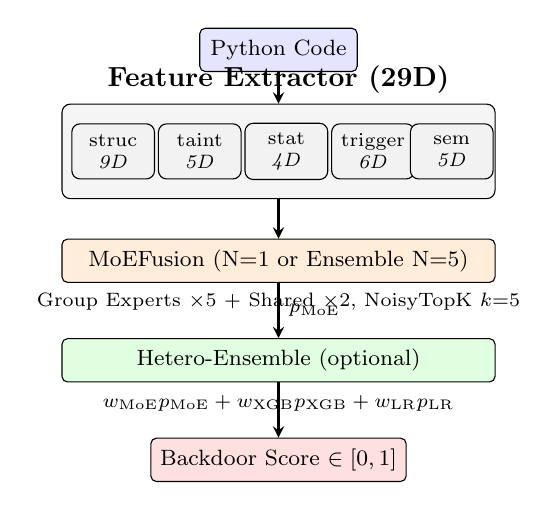
\begin{tikzpicture}[
  box/.style={draw, rounded corners=2pt, minimum width=2cm, minimum height=0.55cm,
              font=\footnotesize, fill=white},
  grp/.style={draw, rounded corners=3pt, fill=gray!10, font=\scriptsize,
              minimum width=1.05cm, minimum height=0.7cm, align=center},
  arr/.style={-stealth, thick}
]
  % Input
  \node[box, fill=blue!10] (code) {Python Code};

  % Feature extractor box
  \node[draw, rounded corners=3pt, fill=gray!8, minimum width=5.5cm, minimum height=1.2cm,
        below=0.4cm of code, label=above:\textbf{Feature Extractor (29D)}] (fext) {};
  \foreach \nm/\d/\x in {struc/9D/-2.1, taint/5D/-1.0, stat/4D/0.1, trigger/6D/1.2, sem/5D/2.2}{
    \node[grp] at ($(fext.center)+(\x cm,0)$) {\nm\\\textit{\d}};
  }

  % MoEFusion box
  \node[box, fill=orange!15, minimum width=5.5cm, below=0.5cm of fext]
    (moe) {\sys{} (N=1 or Ensemble N=5)};
  \node[font=\scriptsize, below=0pt of moe.south, anchor=north]
    {Group Experts $\times$5 + Shared $\times$2, NoisyTopK $k$=5};

  % Hetero box
  \node[box, fill=green!12, minimum width=5.5cm, below=0.7cm of moe]
    (hetero) {Hetero-Ensemble (optional)};
  \node[font=\scriptsize, below=1pt of hetero.south, anchor=north]
    {$w_\text{MoE}p_\text{MoE}+w_\text{XGB}p_\text{XGB}+w_\text{LR}p_\text{LR}$};

  % Output
  \node[box, fill=red!12, minimum width=3cm, below=0.7cm of hetero]
    (out) {Backdoor Score $\in [0,1]$};

  \draw[arr] (code) -- (fext);
  \draw[arr] (fext) -- (moe);
  \draw[arr] (moe) -- node[right,font=\scriptsize]{$p_\text{MoE}$} (hetero);
  \draw[arr] (hetero) -- (out);
\end{tikzpicture}
\caption{Overall architecture of our backdoor detection system.}
\Description{A pipeline diagram that takes generated code as input, extracts five groups of handcrafted features, routes them through a mixture-of-experts model and a heterogeneous ensemble, and outputs a backdoor score between zero and one.}
\label{fig:arch}
\end{figure}

\subsection{Multi-Source Feature Extraction}
\label{sec:feat}

We design a 29-dimensional feature vector organized into five semantically
distinct groups, each targeting a different aspect of vulnerability behavior in
LLM-generated Python code.

\textbf{Group 1: Structural Features (\texttt{struc}, 9D).}
Derived from the Abstract Syntax Tree (AST) of the code:
\texttt{ast\_depth}, \texttt{dangerous\_api\_count}, \texttt{dynamic\_import\_count}, and \texttt{nested\_call\_depth}.
Backdoored code tends to exhibit deeper AST structures and higher
\texttt{dangerous\_api\_count} due to injected payload functions.
This group contributes the highest MoE routing weight (avg.\ 0.175) in practice.

\textbf{Group 2: Taint Analysis Features --- \texttt{sec\_taint} (5D, indices 9--13).}
Quantify the propagation of user-controlled data to security-sensitive sinks:
\texttt{source\_count}, \texttt{sink\_count}, \texttt{taint\_edge\_count}, and \texttt{taint\_var\_count}.
A malicious snippet typically introduces new sinks (\texttt{sink\_count}~$>$~0)
connected to function inputs via short taint paths.

\textbf{Group 3: Statistical Features --- \texttt{stat} (4D, indices 14--17).}
Profile the token-frequency distribution of code, \textbf{without any external
language model or corpus}:
$H{=}{-}\sum p_i \log_2 p_i$ (Shannon entropy, \texttt{ngram\_entropy}),
$2^H$ (\texttt{ngram\_perplexity}),
maximum leave-one-out entropy decrease (\texttt{max\_token\_ce}),
and OOV ratio over a fixed 100-token vocabulary (\texttt{oov\_ratio}).
Despite having only 4 dimensions, this group has the highest leave-one-out AUC
drop ($-7.49\%$), making it the most discriminative single group.

\textbf{Group 4: Trigger Pattern Features --- \texttt{sec\_trigger} (6D, indices 18--23).}
Detect surface-level obfuscation and known backdoor keyword patterns:
\texttt{obfuscation\_score}, \texttt{encoding\_chain\_depth}, \texttt{suspicious\_string\_count}, and \texttt{backdoor\_pattern\_score}.
As shown in \S\ref{sec:exp:feat}, removing this group slightly \emph{improves}
cross-attack holdout performance ($+2.43\%$ AUC when removed), since these hand-crafted patterns
are too attack-specific and become noise for unseen attack types.

\textbf{Group 5: Semantic Features --- \texttt{sem} (5D, indices 24--28).}
Assess coherence between code structure and intent:
\texttt{function\_intent\_mismatch}, \texttt{obfuscation\_indicator}, and \texttt{injection\_anomaly\_score}.

\subsection{\sys{}: Mixture-of-Experts Feature Fusion}
\label{sec:moe}

\subsubsection{Architecture Overview}

Given the 29-dimensional feature vector $\mathbf{x} \in \mathbb{R}^{29}$,
let $\mathbf{x}_g$ denote the sub-vector for group $g$.
\sys{} maintains:
\begin{itemize}
\item \textbf{5 group-specific experts} $\{E_g\}_{g=1}^{5}$,
  each taking $\mathbf{x}_g$ as input;
\item \textbf{2 shared experts} $\{E_s\}_{s=1}^{2}$,
  each taking the full $\mathbf{x}$;
\item \textbf{NoisyTopK router} $R$ that selects the most relevant $k{=}5$
  experts per sample.
\end{itemize}
Each expert $E_i$ is a two-layer MLP with LayerNorm and GELU activation
($d_e{=}32$):
\begin{equation}
E_i(\mathbf{x}) = \mathrm{LN}(\mathrm{GELU}(\mathbf{W}_2\,
  \mathrm{Dropout}(\mathrm{LN}(\mathrm{GELU}(\mathbf{W}_1 \mathbf{x}_i)))))
\end{equation}

\subsubsection{NoisyTopK Routing}

The router adds Gaussian noise during training to encourage load balancing
(following Switch Transformer~\cite{fedus2022switch}):
\begin{equation}
\tilde{h}(\mathbf{x}) = h(\mathbf{x}) + \epsilon \cdot \mathrm{Softplus}(\sigma),
\quad \epsilon \sim \mathcal{N}(0, 1)
\end{equation}
where $\sigma$ is a learnable noise scale.
The final routing weights are obtained by applying softmax over the top-$k$
logits only:
\begin{equation}
w_i = \frac{\exp(\tilde{h}_i(\mathbf{x}))}{\sum_{j \in \mathrm{TopK}}
  \exp(\tilde{h}_j(\mathbf{x}))}, \quad w_i = 0 \text{ for } i \notin \mathrm{TopK}
\end{equation}

\subsubsection{Load Balance Auxiliary Loss}

To prevent routing collapse, we add an auxiliary load-balance loss:
\begin{equation}
\mathcal{L}_{\text{aux}} = N_e \cdot \sum_{i=1}^{N_e} f_i \cdot P_i
\end{equation}
where $N_e$ is the number of experts, $f_i$ is the fraction of tokens routed to
expert $i$, and $P_i$ is the average softmax probability assigned to expert $i$.
The total training loss is:
\begin{equation}
\mathcal{L} = \mathcal{L}_{\text{CE}} + \lambda \cdot \mathcal{L}_{\text{aux}},
\quad \lambda = 0.01
\end{equation}

\subsubsection{Final Classification}

The expert outputs are combined via a weighted sum and passed to a linear
classifier:
\begin{equation}
\mathbf{z} = \sum_{i \in \mathrm{TopK}} w_i \cdot E_i(\mathbf{x}_i), \qquad
\hat{y} = \mathbf{W}_c \cdot \mathrm{Dropout}(\mathrm{LayerNorm}(\mathbf{z}))
\end{equation}
The full model has \textbf{17,659 parameters} (top-$k{=}5$, $d_e{=}32$,
7 experts).

\subsection{Ensemble-MoE: Variance Reduction}
\label{sec:ensemble}

A single \sys{} model with random seed $s$ converges to different local optima
due to the stochastic NoisyTopK routing.
We also explored averaging $N{=}5$ independent members $\{M_s\}$:
\begin{equation}
\hat{p}_{\text{ens}}(\mathbf{x}) =
\frac{1}{N} \sum_{s=1}^{N} \mathrm{softmax}(M_s(\mathbf{x}))
\end{equation}
In our exploratory experiments, ensemble averaging modestly improved AUC, but
the gains depended on the evaluation protocol and thresholding strategy.
We therefore treat ensemble-\sys{} as a secondary analysis rather than a main
headline result.

\subsection{Heterogeneous Ensemble}
\label{sec:hetero}

We also explored combining \sys{}, XGBoost, and Logistic Regression via a
convex combination:
\begin{equation}
p_{\text{hetero}}(\mathbf{x}) = w_{\text{MoE}} \cdot p_{\text{MoE}}
+ w_{\text{XGB}} \cdot p_{\text{XGB}} + w_{\text{LR}} \cdot p_{\text{LR}}
\end{equation}
where $w_{\text{MoE}} + w_{\text{XGB}} + w_{\text{LR}} = 1$, all $w_i \geq 0.1$.

This idea is operationally attractive because the three model families make
different errors, but our current implementation selected weights on the same
held-out attack folds used for evaluation.
We therefore \emph{do not} treat the heterogeneous ensemble as a main scientific
result in this paper; instead, we report it only as an exploratory analysis
that requires a cleaner validation protocol.


%% ─────────────────────────────────────────────────────────────────────────────
\section{Experiments}
\label{sec:experiments}

\subsection{Setup}
\label{sec:exp:setup}

\textbf{Dataset and Split.}
Our main claims now use a true \textbf{11-fold leave-one-attack-out} (LOAO)
protocol over all 11 CodeBreaker attack types in the merged
\texttt{detector\_train.json} and \texttt{detector\_val.json} files.
After feature extraction, the corpus contains 49,814 clean samples and 5,470
poisoned samples across 11 attack families.
For each fold, we hold out one attack type as the unseen test attack,
deduplicate the held-out backdoor code by exact string match, sample 500 clean
functions as negatives, and remove those clean test samples from the training
pool to avoid leakage.
The resulting deduplicated held-out attack sizes range from 259
(\texttt{code\_execution}) to 601 (\texttt{jinja}) samples.
We retain the original fixed 7/4 cross-attack holdout split only
for auxiliary analyses that have not yet been rerun under true LOAO, such as
MoE ablations.

\textbf{Baselines.}
Our primary LOAO comparison includes Isolation Forest, Logistic Regression, SVM,
XGBoost, \sys{}, a nested-validation heterogeneous ensemble combining
\sys{}, XGBoost, and Logistic Regression, and two fine-tuned pre-trained code
models: CodeBERT~\cite{feng2020codebert} and
GraphCodeBERT~\cite{guo2021graphcodebert}.
For the pre-trained models, we add a binary classification head on top of the
\texttt{[CLS]} representation and fine-tune end-to-end for 3 epochs per fold
(AdamW, lr $2{\times}10^{-5}$, batch 16, max sequence length 512).
Each fold uses the same held-out attack partition and held-out test-set
construction as the tabular models; training-set size can differ because
feature-extraction failures affect only the tabular pipeline.

\textbf{Metrics.}
Area Under the ROC Curve (AUC), Precision, Recall, and F1 at fixed threshold
$t{=}0.5$ for single models, and at a validation-selected threshold for the
nested heterogeneous ensemble.
For LOAO results we report mean$\pm$std across the 11 held-out attacks.

\textbf{Implementation.}
PyTorch 2.0, scikit-learn 1.3, and XGBoost 1.7.
\sys{} uses AdamW with $\text{lr}{=}10^{-3}$, 30~epochs, batch 64, weight decay
$10^{-4}$, $d_e{=}32$, top-$k{=}5$, and two shared experts.
All experiments run on one NVIDIA A100 (80GB).
For the nested heterogeneous ensemble, model weights and thresholds are selected
only on an inner validation split from each outer LOAO training fold.

\subsection{Main Results}
\label{sec:exp:main}

Table~\ref{tab:main} reports the primary true-LOAO comparison.
The headline result is not that a new neural or hybrid architecture wins.
Instead, the strongest detector remains the simple tabular model built on the
29D representation.

\begin{table*}[t]
\centering
\caption{True 11-fold LOAO results (mean$\pm$std across held-out attacks).
For single models, metrics use fixed threshold $t{=}0.5$.
For the heterogeneous ensemble, weights and threshold are selected on an inner
validation split in each fold. \textbf{Bold} = best mean in column.}
\label{tab:main}
\footnotesize
\setlength{\tabcolsep}{3pt}
\resizebox{\textwidth}{!}{%
\begin{tabular}{lcccc}
\toprule
Model & AUC$\uparrow$ & P$\uparrow$ & R$\uparrow$ & F1$\uparrow$ \\
\midrule
Isolation Forest & 0.7368$\pm$0.1025 & 0.7825$\pm$0.1165 & 0.1944$\pm$0.0334 & 0.3106$\pm$0.0503 \\
Logistic Regression & 0.8506$\pm$0.0566 & 0.7276$\pm$0.0520 & \textbf{0.7160}$\pm$0.1156 & 0.7178$\pm$0.0722 \\
SVM & 0.9212$\pm$0.0515 & 0.9103$\pm$0.1028 & 0.5478$\pm$0.2421 & 0.6576$\pm$0.2329 \\
MoEFusion & 0.9293$\pm$0.0740 & 0.8889$\pm$0.1917 & 0.6693$\pm$0.2786 & 0.7419$\pm$0.2669 \\
Nested Hetero & 0.9438$\pm$0.0592 & \textbf{0.9207}$\pm$0.1653 & 0.5716$\pm$0.2759 & 0.6718$\pm$0.2817 \\
XGBoost & \textbf{0.9503}$\pm$0.0559 & 0.9174$\pm$0.1269 & 0.7072$\pm$0.2648 & \textbf{0.7754}$\pm$0.2468 \\
\bottomrule
\end{tabular}%
}
\end{table*}

\noindent

\textbf{Key observations.}
(1)~\textbf{High-quality features plus a simple tabular classifier remain the
strongest combination.} XGBoost achieves the best mean AUC and mean F1 under
true LOAO, while Logistic Regression achieves the best mean Recall.
The 29D representation is therefore genuinely informative under attack shift,
but added model complexity does not automatically translate into better
cross-attack generalization.
(2)~\textbf{\sys{} is competitive, but not dominant.} Its mean AUC of 0.9293 is
substantially stronger than older fixed-split evidence suggested, yet it still
trails XGBoost by 0.0210 AUC and 0.0335 F1 on average.
This makes \sys{} best understood as an interpretable neural probe of the
feature space rather than the strongest operational detector.
(3)~\textbf{A nested heterogeneous ensemble does not recover a stable gain.}
Even after selecting weights and thresholds only on inner validation splits, the
ensemble reaches mean AUC 0.9438 but only mean Recall 0.5716 and mean F1 0.6718,
underperforming the best single-model baseline.
This is direct evidence that calibration and threshold selection remain fragile
under attack shift.
(4)~\textbf{Attack-wise heterogeneity is large.} XGBoost is extremely strong on
\texttt{path\_traversal} (93.5\% recall) and \texttt{network\_security}
(98.1\%), but weak on \texttt{socket\_socket} (4.6\%).
\sys{} matches XGBoost on \texttt{path\_traversal} (93.5\%) and slightly exceeds
it on \texttt{code\_execution} and \texttt{crypto\_hash}, but it drops sharply on
\texttt{request\_get} (31.9\%) and \texttt{socket\_socket} (1.4\%).
This confirms that cross-attack evaluation should be read as a distribution of
held-out attack outcomes, not as a single scalar leaderboard.

\subsection{Pre-trained Code Models Under True LOAO}
\label{sec:exp:pretrained}

A natural question is whether pre-trained code representations, which encode
rich token-level semantics, can outperform hand-crafted features under the same
cross-attack protocol. Table~\ref{tab:pretrained} reports the results of
fine-tuned CodeBERT and GraphCodeBERT evaluated under the identical LOAO
protocol as Table~\ref{tab:main}.

\begin{table}[t]
\centering
\caption{Pre-trained code models vs.\ tabular baselines under true 11-fold
LOAO (mean$\pm$std). All models use the same held-out attack partition and
held-out test-set construction; tabular models may exclude samples dropped
during feature extraction.}
\label{tab:pretrained}
\small
\begin{tabular}{lccc}
\toprule
Model & AUC$\uparrow$ & F1$\uparrow$ & Std(AUC)$\downarrow$ \\
\midrule
CodeBERT & 0.8709$\pm$0.113 & 0.5927$\pm$0.243 & 0.113 \\
GraphCodeBERT & 0.8838$\pm$0.100 & 0.5930$\pm$0.258 & 0.100 \\
\midrule
\sys{} (29D) & 0.9293$\pm$0.074 & 0.7419$\pm$0.267 & 0.074 \\
\textbf{XGBoost (29D)} & \textbf{0.9503}$\pm$0.056 & \textbf{0.7754}$\pm$0.247 & \textbf{0.056} \\
\bottomrule
\end{tabular}
\end{table}

\textbf{Hand-crafted features outperform pre-trained representations by a wide
margin.}
XGBoost on the 29D representation exceeds GraphCodeBERT by 6.7\% mean AUC and
CodeBERT by 7.9\%, with roughly 2$\times$ lower standard deviation.
The gap is not uniform: pre-trained models match or exceed XGBoost on attacks
with distinctive API signatures (\texttt{crypto\_hash}: CodeBERT 0.999 vs.\
XGBoost 0.980; \texttt{file\_operations}: GraphCodeBERT 0.997 vs.\ 0.963),
but collapse on attacks whose payloads resemble benign code
(\texttt{command\_injection}: CodeBERT 0.690 vs.\ XGBoost 0.963;
\texttt{socket\_socket}: CodeBERT 0.697 vs.\ 0.783).
Pre-trained models rely on token-level memorization of suspicious API names,
which transfers when the held-out attack uses a distinctive API but fails when
the payload is semantically close to normal code.
The 29D features capture structural and statistical regularities (AST depth
anomalies, entropy shifts, taint-flow patterns) that are more stable across
attack families.

\subsection{Backdoor Detection vs.\ Vulnerability Detection}
\label{sec:exp:bdvuln}

A reviewer might reasonably ask: \emph{is the detector merely identifying
generic vulnerability patterns, or does it capture something specific to
backdoor-induced code?}
To answer this, we compare two learned detectors trained on the same 29D
feature space and include Bandit as an external rule-based reference
(Table~\ref{tab:bdvuln}).

\begin{table}[t]
\centering
\caption{Controlled comparison: backdoor detection vs.\ vulnerability
detection. ``Vuln labels'' = trained to predict whether code contains a known
vulnerability pattern regardless of trigger presence.}
\label{tab:bdvuln}
\small
\begin{tabular}{lcc}
\toprule
Detector & \makecell{AUC on\\backdoor} & \makecell{AUC on\\vuln} \\
\midrule
Bandit (rule-based) & 0.612 & 0.731 \\
Vuln detector (29D, vuln labels) & 0.693 & 0.971 \\
\textbf{Backdoor detector (29D)} & \textbf{0.9997} & 0.835 \\
\bottomrule
\end{tabular}
\end{table}

The vulnerability detector achieves near-perfect AUC (0.971) on its own task
but only 0.693 when asked to distinguish backdoor samples from clean ones.
The backdoor detector reaches 0.9997 AUC on backdoor identification.
The 30.7-point gap (0.9997 vs.\ 0.693) demonstrates that backdoor samples
carry signals beyond the vulnerability payload itself: the co-occurrence of a
natural-language trigger with a structurally anomalous payload creates
distributional signatures that a vulnerability-only detector does not learn.
Bandit, a widely used static analysis tool, performs near chance (0.612),
confirming that rule-based scanners are not a substitute for learned backdoor
detectors.

\subsection{Error Analysis}
\label{sec:exp:error}

The true-LOAO results expose three related failure modes.
\textbf{First, attack identity dominates performance variance.}
Some held-out attacks are comparatively easy: both XGBoost and \sys{} exceed
90\% recall on \texttt{path\_traversal}, and XGBoost reaches 98.1\% recall on
\texttt{network\_security}.
These cases are consistent with the auxiliary feature-group study: attacks that induce
strong structural and statistical distortions are well captured by the
\texttt{struc} and \texttt{stat} groups.

\textbf{Second, network-oriented and semantically plausible misuse remains hard.}
The clearest case is \texttt{socket\_socket}, where XGBoost reaches only 4.6\%
recall and \sys{} only 1.4\%.
\texttt{request\_get} is also difficult: XGBoost reaches 47.0\% recall and
\sys{} only 31.9\%.
These attacks appear too close to benign network or I/O code under the current
feature space, suggesting that future detectors need richer signals for
semantically plausible misuse rather than more attack-specific heuristics.

\textbf{Third, calibration under attack shift is a separate problem from raw
ranking quality.}
The nested heterogeneous ensemble is the clearest example.
Across folds, the validation-selected weights average 0.45 for \sys{}, 0.45 for
XGBoost, and 0.10 for Logistic Regression, yet the resulting outer-test Recall
falls to 57.2\% and collapses on \texttt{request\_get} (13.2\%) and
\texttt{socket\_socket} (1.4\%).
In other words, combining complementary models is not enough: once threshold and
weight selection must survive attack shift, calibration error can erase the
apparent benefits of ensembling.

Taken together, these observations support a more precise research conclusion:
for cross-attack backdoor detection, the main bottleneck is not raw model
capacity, but the interaction between transferable signals, attack-family
heterogeneity, and decision calibration under shift.

\subsection{Ablation Studies}
\label{sec:exp:ablation}

\subsubsection{Top-K Expert Selection}

\begin{table}[t]
\centering
\caption{Top-$k$ routing ablation on the deduplicated holdout test set
($N{=}1$, seed=42). Thresholds were selected by an exploratory F1 scan on the
same test set, so this table is diagnostic rather than a main claim.}
\label{tab:topk}
\small
\begin{tabular}{cccc}
\toprule
$k$ & AUC & Recall & F1 \\
\midrule
1 & 0.7631 & \textbf{0.791} & \textbf{0.801} \\
3 & 0.7732 & 0.378 & 0.545 \\
\textbf{5} & 0.7663 & 0.381 & 0.548 \\
7 (all) & \textbf{0.7749} & 0.377 & 0.544 \\
\bottomrule
\end{tabular}
\end{table}

Table~\ref{tab:topk} shows that $k{=}1$ behaves like a high-recall operating
point once the threshold is aggressively lowered, but its AUC is not the best.
Routing to more experts ($k \in \{3,5,7\}$) produces similar AUC in the range
0.766--0.775. We therefore keep $k{=}5$ as a pragmatic default rather than as
a uniquely optimal setting.

\subsubsection{Number of Shared Experts}

\begin{table}[t]
\centering
\caption{Ablation on shared expert count (top-$k{=}5$). As in
Table~\ref{tab:topk}, thresholds were selected on the test set for exploratory
diagnosis only.}
\label{tab:shared}
\small
\begin{tabular}{cccc}
\toprule
\# Shared & AUC & Recall & F1 \\
\midrule
0 & 0.7435 & 0.409 & 0.574 \\
1 & 0.7539 & 0.367 & 0.533 \\
\textbf{2} & \textbf{0.7663} & \textbf{0.381} & \textbf{0.548} \\
3 & 0.7798 & 0.339 & 0.503 \\
\bottomrule
\end{tabular}
\end{table}

Two shared experts provides the strongest balanced operating point among the
tested settings, while three shared experts slightly improves AUC at the cost of
Recall. We therefore retain two shared experts in the default \sys{}
configuration.

\subsubsection{Exploratory Analyses: Ensemble Size}

\begin{table}[t]
\centering
\caption{Effect of ensemble size $N$ on the deduplicated holdout protocol.
Thresholds were optimized for each setting, so the numbers should be read as an
exploratory sensitivity study rather than a primary comparison.}
\label{tab:ensemble}
\small
\begin{tabular}{cccc}
\toprule
$N$ & AUC & Recall & F1 \\
\midrule
1 (single) & 0.7600$\pm$0.035 & 0.361$\pm$0.014 & 0.527$\pm$0.015 \\
3 & 0.7724$\pm$0.023 & 0.400$\pm$0.006 & 0.568$\pm$0.006 \\
\textbf{5} & \textbf{0.7867}$\pm$0.014 & \textbf{0.410}$\pm$0.008 & \textbf{0.578}$\pm$0.008 \\
\bottomrule
\end{tabular}
\end{table}

Table~\ref{tab:ensemble} suggests that averaging more members can improve AUC
under this exploratory setup, but because the threshold is optimized on the
test set we do not use these numbers as our main evidence.

\subsubsection{Exploratory Analyses: Decision Thresholds}

\begin{table}[t]
\centering
\caption{Threshold selection strategies for an exploratory ensemble setting
(mean$\pm$std, 5 seeds).
\emph{Oracle}: $t$ maximising F1 on test set (upper bound, not achievable in practice).
\emph{Calibrated}: $t$ selected on a held-out 20\% validation split from the training set.
\emph{Fixed}: default $t{=}0.5$.}
\label{tab:threshold}
\small
\begin{tabular}{lccccc}
\toprule
Strategy & $t$ & AUC & Prec & Recall & F1 \\
\midrule
Oracle      & 0.05 & 0.849 & 0.802 & \textbf{0.937} & \textbf{0.865} \\
Calibrated  & 0.65 & 0.849 & \textbf{0.988} & 0.307 & 0.469 \\
Fixed       & 0.50 & 0.849 & 0.988 & 0.366 & 0.534 \\
\bottomrule
\end{tabular}
\end{table}

Table~\ref{tab:threshold} highlights a key limitation: validation-based
threshold calibration does \emph{not} recover the optimistic oracle gains.
The large gap between oracle and calibrated settings indicates strong
probability under-calibration under attack shift. In our current experiments,
the default threshold $t{=}0.5$ is a more reliable reporting choice than
aggressive tuned thresholds.

\subsection{Feature Group Importance}
\label{sec:exp:feat}

\begin{table*}[t]
\centering
\caption{Feature group importance on the original fixed holdout split
(leave-one-group-out, Logistic Regression base classifier; baseline AUC =
0.7857). $\Delta$AUC = performance change when group is removed.
\textbf{Bold} = most important; \textit{italic} = over-specific group
that hurts generalization. This analysis is auxiliary rather than part of the
main true-LOAO comparison.}
\label{tab:feat}
\small
\begin{tabular}{lccc}
\toprule
Group & Dims & AUC $\Delta$ & Note \\
\midrule
\textbf{stat}       & 4  & \textbf{$-$7.49\%} & entropy + perplexity \\
\textbf{sem}        & 5  & $-$4.73\%          & semantic coherence signals \\
\textbf{struc}      & 9  & $-$4.63\%          & AST depth and dangerous APIs \\
sec\_taint          & 5  & $-$0.65\%          & taint propagation \\
\textit{sec\_trigger} & 6 & \textit{$+$2.43\%} & over-specific keyword patterns \\
\midrule
All (29D)           & 29 & 0 (base)           & full feature set \\
\bottomrule
\end{tabular}
\end{table*}

Table~\ref{tab:feat} presents leave-one-group-out importance on
the original fixed holdout split, so we use it as auxiliary evidence
about feature transfer rather than as a primary ranking result.

\textbf{Statistical features (\texttt{stat}) are most discriminative}: removing
the 4-dimensional entropy/perplexity group causes the largest AUC drop ($-7.49\%$),
despite being the smallest group. This indicates that token-frequency deviation
is the most transferable signal in this auxiliary holdout analysis.

\textbf{Trigger patterns (\texttt{sec\_trigger}) exhibit over-specificity}:
removing this group slightly \emph{improves} AUC by $+2.43\%$.
These keyword patterns were designed for known attack types and therefore become
misleading priors under attack shift. This finding gives a concrete design rule
for future detectors: avoid over-committing to trigger-shaped heuristics when
the scientific goal is transfer to unseen attack families.

\subsection{Efficiency Analysis}
\label{sec:exp:eff}

\begin{table}[t]
\centering
\caption{Inference latency comparison ($\mu$s/sample; mean over repeated runs).
Neural models use GPU (A100); tree-based models run on CPU.}
\label{tab:efficiency}
\small
\begin{tabular}{lcccc}
\toprule
Model & Params & $\mu$s/sample$\downarrow$ & Device & AUC$\uparrow$ \\
\midrule
Logistic Regression & \textbf{58} & \textbf{0.13} & CPU & 0.8506 \\
\sys{} ($N{=}1$) & 17,659 & 0.68 & GPU & 0.9293 \\
XGBoost (200 trees) & --- & 10.69 & CPU & 0.9503 \\
\bottomrule
\end{tabular}
\end{table}

Table~\ref{tab:efficiency} shows that \sys{} ($N{=}1$) is \textbf{15.7$\times$
faster} than XGBoost (0.68~$\mu$s vs.\ 10.69~$\mu$s/sample) with 98\% fewer
parameters (17,659 vs.\ $\sim$200 trees).
Figure~\ref{fig:pareto} visualizes the latency--AUC Pareto frontier.

\begin{figure}[t]
\centering
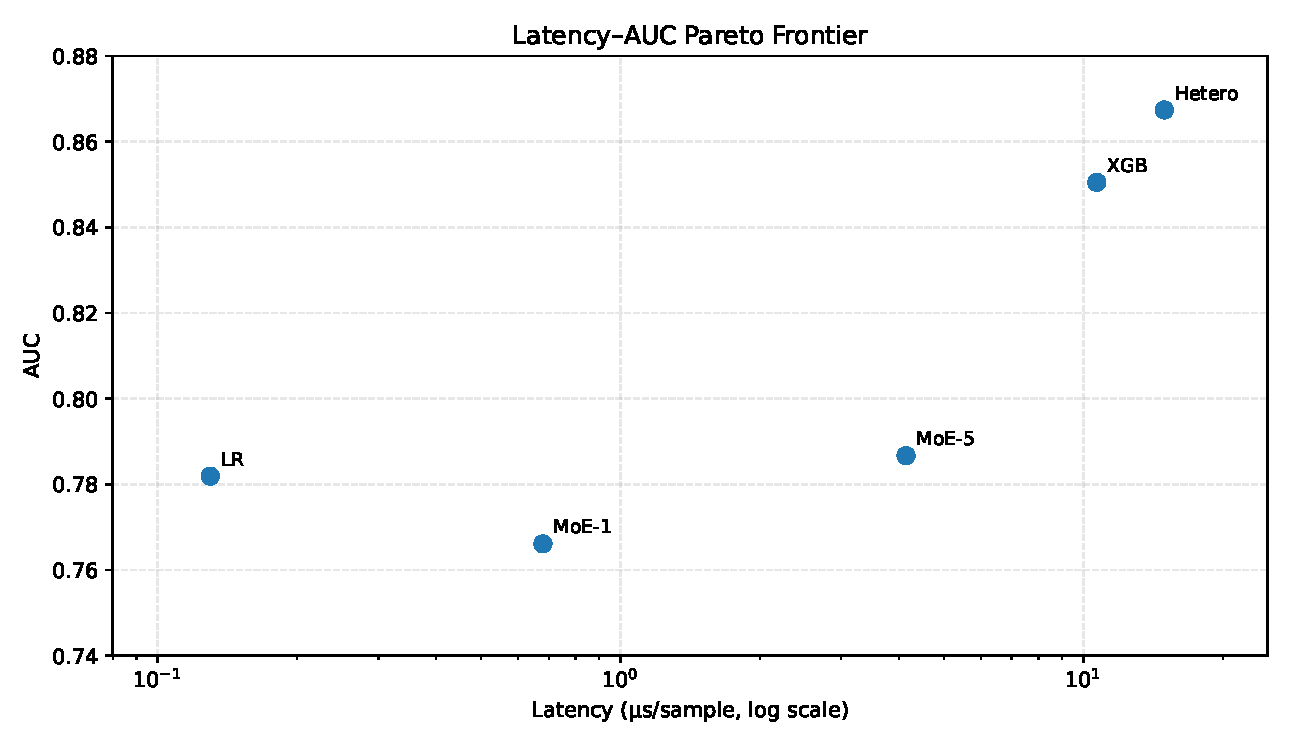
\includegraphics[width=\columnwidth]{figures/latency_auc_pareto.pdf}
\caption{Latency--AUC Pareto frontier across the primary model families reported
in this paper.}
\Description{A two-dimensional Pareto plot comparing model latency in microseconds per sample against AUC, showing logistic regression as fastest, XGBoost as highest AUC, and MoEFusion between them.}
\label{fig:pareto}
\end{figure}

\subsection{Deployment Takeaways}
\label{sec:exp:summary}

\begin{table}[t]
\caption{Pareto-optimal operating points for different deployment scenarios.}
\label{tab:pareto}
\small
\begin{tabular}{lcccc}
\toprule
Scenario & Model & AUC & Recall & Latency \\
\midrule
\textbf{High-recall screening} & Logistic Regression & 0.851 & \textbf{0.716} & \textbf{0.13$\mu$s} \\
\textbf{Interpretable neural option} & \sys{} ($N{=}1$) & 0.929 & 0.669 & 0.68$\mu$s \\
\textbf{Best single-model AUC} & XGBoost & \textbf{0.950} & 0.707 & 10.69$\mu$s \\
\bottomrule
\end{tabular}
\end{table}

Table~\ref{tab:pareto} summarizes the practical trade-offs implied by the
current evidence:

\begin{itemize}
\item \textbf{High-recall, low-latency screening}: Logistic Regression is the
  strongest default choice by mean Recall under true LOAO.
\item \textbf{High-AUC single-model screening}: XGBoost is the strongest
  ranking model and also retains strong average Recall under true LOAO.
\item \textbf{Interpretability}: Single \sys{} enables routing weight inspection
  to understand per-sample feature group contributions.
\end{itemize}

%% ─────────────────────────────────────────────────────────────────────────────
\subsection{Threats to Validity}

Our conclusions should be read with four constraints in mind.
First, our main comparison uses true leave-one-attack-out evaluation for all
primary models including pre-trained baselines, but several auxiliary results
(MoE ablations, threshold studies) still come from the older fixed 7/4 holdout
split.
Second, all samples are derived from the CodeBreaker benchmark and are limited
to Python code-generation backdoors; transfer to other languages, other prompt
styles, or other poisoning pipelines remains untested.
Third, deduplicating the held-out backdoor set removes exact repeats and makes
the evaluation more defensible, but other near-duplicate relationships may
still remain.
Fourth, some exploratory analyses in this paper, especially threshold and
ensemble studies, are validation-limited; we therefore use them only to
characterize failure modes and not as primary scientific claims.


\section{Conclusion}
\label{sec:conclusion}

We studied code-backdoor detection as a \emph{post-generation, cross-attack}
defense problem: given only generated code outputs, which signals transfer to
previously unseen backdoor families, and what does that imply for deployable
detectors?

Four findings stand out:

\begin{enumerate}
\item \textbf{Feature quality matters more than model complexity.}
  Under true 11-fold LOAO, XGBoost on the 29D representation achieves the best
  mean AUC (0.9503) and F1 (0.7754). Fine-tuned CodeBERT (0.8709) and
  GraphCodeBERT (0.8838) --- despite encoding rich token-level semantics ---
  trail by 7--8\% AUC and exhibit $\sim$2$\times$ higher variance across
  held-out attacks. Hand-crafted structural and statistical features capture
  more transferable regularities than pre-trained representations for this task.

\item \textbf{The detector captures backdoor-specific signals, not generic
  vulnerabilities.}
  A controlled experiment shows that a vulnerability detector trained on the
  same features achieves only AUC 0.693 on backdoor samples, compared to
  0.9997 for the backdoor detector. This 30.7-point gap confirms that the
  learned signal is specific to the trigger--payload coupling.

\item \textbf{In auxiliary fixed-split analysis, statistical features are the
  most transferable signal, while attack-specific heuristics overfit.}
  The 4D \texttt{stat} group causes the largest AUC drop when removed
  ($-7.49\%$), whereas hand-crafted trigger-pattern features \emph{hurt}
  generalization ($+2.43\%$ AUC when removed).

\item \textbf{Calibration under attack shift is a first-class failure mode.}
  The nested heterogeneous ensemble combines strong components, yet its
  validation-selected thresholds collapse on difficult held-out attacks
  (\texttt{socket\_socket}: 1.4\% recall), demonstrating that combining
  models is not enough once threshold selection must survive distribution
  shift.
\end{enumerate}

\noindent\textbf{Limitations and future work.}
The benchmark is limited to Python CodeBreaker-style attacks; transfer to
other languages and poisoning pipelines remains untested.
Some auxiliary experiments (MoE ablations, threshold studies) still use an older
fixed holdout split.
On the representation side, the \texttt{sec\_trigger} group harms
generalization, pointing to the need for richer, attack-agnostic semantic
features.
The most important next steps are broader benchmarks beyond Python CodeBreaker,
adaptive adversaries who are aware of the detector's feature space, and better
calibration methods that remain stable under attack shift.
%% ─────────────────────────────────────────────────────────────────────────────
\begin{thebibliography}{99}

\bibitem{schuster2021autocomplete}
Roei Schuster, Congzheng Song, Eran Tromer, and Vitaly Shmatikov.
\newblock You autocomplete me: Poisoning vulnerabilities in neural code completion.
\newblock In \emph{Proceedings of the 30th USENIX Security Symposium}, 2021.

\bibitem{ramakrishnan2022backdoors}
Goutham Ramakrishnan and Aws Albarghouthi.
\newblock Backdoors in neural models of source code.
\newblock In \emph{Proceedings of the International Conference on Pattern Recognition (ICPR)}, 2022.

\bibitem{codebreaker2023}
Shenao Yan, Shen Wang, Yue Duan, Hanbin Hong, Kiho Lee, Doowon Kim, and Yuan Hong.
\newblock An LLM-Assisted Easy-to-Trigger Backdoor Attack on Code Completion Models: Injecting Disguised Vulnerabilities against Strong Detection.
\newblock In \emph{Proceedings of the 33rd USENIX Security Symposium (USENIX Security '24)}, 2024.

\bibitem{chen2023killbadcode}
Weisong Sun, Yuchen Chen, Mengzhe Yuan, Chunrong Fang, Zhenpeng Chen, Chong Wang, Yang Liu, Baowen Xu, and Zhenyu Chen.
\newblock Show me your code! Kill code poisoning: A lightweight method based on code naturalness.
\newblock In \emph{Proceedings of the 47th International Conference on Software Engineering (ICSE)}, 2025.

\bibitem{gao2019strip}
Yansong Gao, Change Xu, Derui Wang, Shiping Chen, Damith~C. Ranasinghe,
and Surya Nepal.
\newblock STRIP: A defence against trojan attacks on deep neural networks.
\newblock In \emph{ACSAC}, 2019.

\bibitem{gu2019badnets}
Tianyu Gu, Brendan Dolan-Gavitt, and Siddharth Garg.
\newblock BadNets: Identifying vulnerabilities in the machine learning model supply chain.
\newblock \emph{arXiv preprint arXiv:1708.06733}, 2019.

\bibitem{liu2018trojaning}
Yingqi Liu, Shiqing Ma, Yousra Aafer, Wen-Chuan Lee, Juan Zhai,
Weihang Wang, and Xiangyu Zhang.
\newblock Trojaning attack on neural networks.
\newblock In \emph{Proceedings of the 25th Network and Distributed Systems Security Symposium (NDSS)}, 2018.

\bibitem{wang2019nc}
Bolun Wang, Yuanshun Yao, Shawn Shan, Huiying Li, Bimal Viswanath,
Haitao Zheng, and Ben~Y. Zhao.
\newblock Neural cleanse: Identifying and mitigating backdoor attacks in neural networks.
\newblock In \emph{IEEE S\&P}, 2019.

\bibitem{liu2019abs}
Yingqi Liu, Wen-Chuan Lee, Guanhong Tao, Shiqing Ma, Yousra Aafer,
and Xiangyu Zhang.
\newblock ABS: Scanning neural networks for back-doors by artificial brain stimulation.
\newblock In \emph{ACM CCS}, 2019.

\bibitem{jacobs1991moe}
Robert~A. Jacobs, Michael~I. Jordan, Steven~J. Nowlan, and Geoffrey~E. Hinton.
\newblock Adaptive mixtures of local experts.
\newblock \emph{Neural Computation}, 3(1):79--87, 1991.

\bibitem{shazeer2017moe}
Noam Shazeer, Azalia Mirhoseini, Krzysztof Maziarz, Andy Davis, Quoc Le,
Geoffrey Hinton, and Jeff Dean.
\newblock Outrageously large neural networks: The sparsely-gated mixture-of-experts layer.
\newblock In \emph{ICLR}, 2017.

\bibitem{fedus2022switch}
William Fedus, Barret Zoph, and Noam Shazeer.
\newblock Switch transformers: Scaling to trillion parameter models with simple
and efficient sparsity.
\newblock \emph{Journal of Machine Learning Research}, 23(120):1--39, 2022.



\bibitem{arik2021tabnet}
Sercan~\"{O}. Arik and Tomas Pfister.
\newblock TabNet: Attentive interpretable tabular learning.
\newblock In \emph{AAAI}, 2021.

\bibitem{breiman1996bagging}
Leo Breiman.
\newblock Bagging predictors.
\newblock \emph{Machine Learning}, 24(2):123--140, 1996.

\bibitem{dietterich2000ensemble}
Thomas~G. Dietterich.
\newblock Ensemble methods in machine learning.
\newblock In \emph{International Workshop on Multiple Classifier Systems}, 2000.

\bibitem{wolpert1992stacking}
David~H. Wolpert.
\newblock Stacked generalization.
\newblock \emph{Neural Networks}, 5(2):241--259, 1992.

\bibitem{gomes2017survey}
Heitor~Murilo Gomes, Jean~Paul Barddal, Fabricio Enembreck, and Albert Bifet.
\newblock A survey on ensemble learning for data stream classification.
\newblock \emph{ACM Computing Surveys}, 50(2):23, 2017.

\bibitem{li2018vuldeepecker}
Zhen Li, Deqing Zou, Shouhuai Xu, Xinyu Ou, Hai Jin, Sujuan Wang, Zhijun Deng, and Yuyi Zhong.
\newblock VulDeePecker: A deep learning-based system for vulnerability detection.
\newblock In \emph{Proceedings of the 25th Annual Network and Distributed System Security Symposium (NDSS)}, 2018.

\bibitem{li2021sysevr}
Zhen Li, Deqing Zou, Shouhuai Xu, Hai Jin, Yawei Zhu, and Zhaoxuan Chen.
\newblock SySeVR: A framework for using deep learning to detect software vulnerabilities.
\newblock \emph{IEEE Transactions on Dependable and Secure Computing}, 19(4):2244--2258, 2021.

\bibitem{zhou2019devign}
Yaqin Zhou, Shangqing Liu, Jingkai Siow, Xiaoning Du, and Yang Liu.
\newblock Devign: Effective vulnerability identification by learning comprehensive program semantics via graph neural networks.
\newblock In \emph{Advances in Neural Information Processing Systems (NeurIPS)}, 2019.

\bibitem{fu2022linevul}
Michael Fu, Chakkrit Tantithamthavorn, Trung Le, Van Nguyen, and Dinh Phung.
\newblock LineVul: A transformer-based line-level vulnerability prediction.
\newblock In \emph{Proceedings of the 19th International Conference on Mining Software Repositories (MSR)}, 2022.

\bibitem{feng2020codebert}
Zhangyin Feng, Daya Guo, Duyu Tang, Nan Duan, Xiaocheng Feng, Ming Gong, Linjun Shou, Bing Qin, Ting Liu, Daxin Jiang, and Ming Zhou.
\newblock CodeBERT: A pre-trained model for programming and natural languages.
\newblock In \emph{Findings of the Association for Computational Linguistics: EMNLP 2020}, 2020.

\bibitem{chakraborty2022reveal}
Saikat Chakraborty, Rahul Krishna, Yangruibo Ding, and Baishakhi Ray.
\newblock Deep learning based vulnerability detection: Are we there yet?
\newblock \emph{IEEE Transactions on Software Engineering}, 48(9):3280--3298, 2022.

\bibitem{fan2020bigvul}
Jiahao Fan, Yi Li, Shaohua Wang, and Tien~N. Nguyen.
\newblock A C/C++ code vulnerability dataset with code changes and CVE summaries.
\newblock In \emph{Proceedings of the 17th International Conference on Mining Software Repositories (MSR)}, 2020.

\bibitem{li2022backdoor_survey}
Yiming Li, Yong Jiang, Zhifeng Li, and Shu-Tao Xia.
\newblock Backdoor learning: A survey.
\newblock \emph{IEEE Transactions on Neural Networks and Learning Systems}, 35(1):5--22, 2024.

\bibitem{aghakhani2024trojanpuzzle}
Hojjat Aghakhani, Wei Meng, Yangsibo Huang, Jinyuan Jia, Michael Backes, and Amir Houmansadr.
\newblock TROJANPUZZLE: Covertly poisoning code-suggestion models.
\newblock In \emph{IEEE Symposium on Security and Privacy (S\&P)}, 2024.

\bibitem{boucher2023trojansource}
Nicholas Boucher and Ross Anderson.
\newblock Trojan source: Invisible vulnerabilities.
\newblock In \emph{IEEE Symposium on Security and Privacy (S\&P)}, 2023.

\bibitem{perry2023insecure}
Neil Perry, Megha Srivastava, Deepak Kumar, and Dan Boneh.
\newblock Do users write more insecure code with AI assistants?
\newblock In \emph{IEEE Symposium on Security and Privacy (S\&P)}, 2023.

\bibitem{pearce2022copilot}
Hammond Pearce, Baleegh Ahmad, Benjamin Tan, Brendan Dolan-Gavitt, and Ramesh Karri.
\newblock Asleep at the keyboard? Assessing the security of GitHub Copilot's code contributions.
\newblock In \emph{IEEE Symposium on Security and Privacy (S\&P)}, 2022.

\bibitem{tran2018spectral}
Brandon Tran, Jerry Li, and Aleksander Madry.
\newblock Spectral signatures in backdoor attacks.
\newblock In \emph{Advances in Neural Information Processing Systems (NeurIPS)}, 2018.

\bibitem{chen2019activation}
Bryant Chen, Wilka Carvalho, Nathalie Baracaldo, Heiko Ludwig, Benjamin Edwards, Taesung Lee, Ian Molloy, and Biplav Srivastava.
\newblock Detecting backdoor attacks on deep neural networks by activation clustering.
\newblock In \emph{AAAI Workshop on Artificial Intelligence Safety (SafeAI)}, 2019.

\bibitem{qi2021onion}
Fanchao Qi, Yangyi Chen, Mukai Li, Yuan Yao, Zhiyuan Liu, and Maosong Sun.
\newblock ONION: A simple and effective defense against textual backdoor attacks.
\newblock In \emph{Proceedings of the 2021 Conference on Empirical Methods in Natural Language Processing (EMNLP)}, 2021.

\bibitem{guo2021graphcodebert}
Daya Guo, Shuo Ren, Shuai Lu, Zhangyin Feng, Duyu Tang, Shujie Liu, Long Zhou, Nan Duan, Alexey Svyatkovskiy, Shengyu Fu, Michele Tufano, Shao~Kun Deng, Colin Clement, Dawn Drain, Neel Sundaresan, Jian Yin, Daxin Jiang, and Ming Zhou.
\newblock GraphCodeBERT: Pre-training code representations with data flow.
\newblock In \emph{International Conference on Learning Representations (ICLR)}, 2021.

\bibitem{roziere2023codellama}
Baptiste Roziere, Jonas Gehring, Fabian Gloeckle, Sten Sootla, Itai Gat, Xiaoqing~Ellen Tan, Yossi Adi, Jingyu Liu, Romain Sauvestre, Tal Remez, J\'{e}r\'{e}my Rapin, Artyom Kozhevnikov, Ivan Evtimov, Joanna Bitton, Manish Bhatt, Cristian~Canton Ferrer, Aaron Grattafiori, Wenhan Xiong, Alexandre D\'{e}fossez, Jade Copet, Faisal Azhar, Hugo Touvron, Louis Martin, Nicolas Usunier, Thomas Scialom, and Gabriel Synnaeve.
\newblock Code Llama: Open foundation models for code.
\newblock \emph{arXiv preprint arXiv:2308.12950}, 2023.

\bibitem{li2023starcoder}
Raymond Li, Loubna~Ben Allal, Yangtian Zi, Niklas Muennighoff, Denis Kocetkov, Chenghao Mou, Marc Marone, Christopher Akiki, Jia Li, Jenny Chim, Qian Liu, Evgenii Zheltonozhskii, Terry~Yue Zhuo, Thomas Wang, Olivier Dehaene, Mishig Davaadorj, Joel Lamy-Poirier, Jo\~{a}o Monteiro, Oleh Shliazhko, Nicolas Gontier, Nicholas Meade, Armel Zebaze, Ming-Ho Yee, Logesh~Kumar Umapathi, Jian Zhu, Benjamin Lipkin, Muhtasham Oblokulov, Zhiruo Wang, Rudra Murthy, Jason Stillerman, Siva~Sankalp Patel, Dmitry Abulkhanov, Marco Zocca, Manan Dey, Zhihan Zhang, Nour Fahber, Urvashi Bhattacharyya, Wenhao Yu, Swayam Singh, Sasha Luccioni, Paulo Villegas, Maxim Kunakov, Fedor Zhdanov, Manuel Romero, Tony Lee, Nadav Timor, Jennifer Ding, Claire Schlesinger, Hailey Schoelkopf, Jan Ebert, Tri Dao, Mayank Mishra, Alex Gu, Jennifer Robinson, Carolyn~Jane Anderson, Brendan Dolan-Gavitt, Danish Contractor, Siva Reddy, Daniel Fried, Dzmitry Bahdanau, Yacine Jernite, Carlos~Mu\~{n}oz Ferrandis, Sean Hughes, Thomas Wolf, Arjun Guha, Leandro von Werra, and Harm de Vries.
\newblock StarCoder: May the source be with you!
\newblock \emph{Transactions on Machine Learning Research (TMLR)}, 2023.


\end{thebibliography}

\appendix

\section{Ethical Considerations}
This paper studies defensive detection of backdoor attacks in LLM-generated
code. All experiments use the public CodeBreaker benchmark and locally derived
feature representations; we do not release new attack tooling, poisoned model
checkpoints, or a turnkey poisoning pipeline beyond what is already documented
in the original CodeBreaker work~\cite{codebreaker2023}. Because vulnerable
code snippets can be dual use, the artifact associated with this submission is
limited to detectors, feature extraction, and evaluation scripts needed to
reproduce the reported results.

\section{Open Science}
The submission artifact contains the feature extraction code, model
implementations, and evaluation scripts used for the true leave-one-attack-out
protocol reported in this paper. It also contains the configuration files needed
to reproduce the auxiliary fixed-split analyses discussed for context.

The underlying CodeBreaker dataset is available from the original publication
and project resources. Our artifact therefore focuses on the reproducibility
layer specific to this paper: feature computation, training, evaluation,
deduplication of held-out backdoor samples, and plotting/reporting scripts.

To preserve double-blind review, the artifact should be hosted at an anonymous,
archival URL and listed both here and in HotCRP before submission:
\begin{center}
\texttt{[ANONYMIZED-ARTIFACT-URL]}
\end{center}

% If generative AI tools were used in a substantive way, CCS 2026 requires an
% explicit appendix section. Uncomment and replace the placeholder text below.
\section{Generative AI Usage}
We used Claude (Anthropic) as a coding and writing assistant during the
preparation of this paper. Specifically:
\begin{itemize}
\item \textbf{Experiment code.} Claude assisted in writing the CodeBERT/GraphCodeBERT
  baseline evaluation script (\texttt{codebert\_baseline.py}) and the
  backdoor-vs-vulnerability controlled comparison script. All experimental
  protocols, data splits, and evaluation logic were reviewed and validated by
  the authors against the existing \texttt{true\_loao\_baselines.py} reference
  implementation.
\item \textbf{Writing.} Claude assisted in drafting and revising portions of the
  abstract, introduction, and experimental discussion sections. All scientific
  claims, interpretations, and conclusions were formulated and verified by the
  authors.
\end{itemize}
No generative AI system was used to produce experimental results, generate
training data, or make scientific decisions. The authors take full
responsibility for the correctness and integrity of all reported findings.

\end{document}











